\chapter{Implementation and Fabrication}\label{ch:implementation}
RayGuard involves no physical hardware build. Its fabrication-equivalent work is
the construction of the software pipeline and operator application, the
collection of the X-ray dataset, and the verification records that support each
claim. This chapter describes the implemented software (Section~\ref{sec:software}),
the dataset audit and collection (Section~\ref{sec:data}), the verification
results (Section~\ref{sec:verification}), the evaluation protocol and the executed
fine-tuning study (Section~\ref{sec:protocol}), the resulting prototype detection
results (Section~\ref{sec:results}), a walkthrough of the application
(Section~\ref{sec:walkthrough}), and the remaining application acceptance
(Section~\ref{sec:acceptance}).

%-----------------------------------------------------------------------------
\section{Software Implementation}\label{sec:software}

\subsection{Implemented Components}
The software is split between the research repository, which holds the shared
engine, contracts and research tools, and the application repository, which holds
the operator interface. Table~\ref{tab:components-sw} lists the components, the
pull request or commit through which each entered the code base, and the level of
evidence behind it.

\begin{table}[htbp]
\centering\tablesetup
\caption{Implemented software components.}
\label{tab:components-sw}
\begin{tabularx}{\textwidth}{@{}L{0.22\textwidth}YL{0.2\textwidth}L{0.17\textwidth}@{}}
\toprule
Component & Function & Integration & Evidence\\
\midrule
Audit tools & Decode images and check COCO annotations, splits and box geometry &
Research repository, \file{main} & Executed on IEDXray\\
Run contract and baseline adapter & Validate saved predictions against the run
manifest and the task class map & PRs~\#17, \#19 & Synthetic tests; CI\\
Evaluator & Convert boxes to COCO format and compute AP and AR under a frozen
protocol & PR~\#18 (\file{9350482}) & Synthetic tests; CI\\
Initialization receipt & Hash the YOLOv10-M starting weights and reject a
mismatch & PR~\#21 (\file{29d6d0f}) & Synthetic tests; CI\\
Box repair & Clamp five sub-pixel training boxes in a derived copy with a change
record & PRs~\#22, \#24 & Executed on the training exports\\
Training workflow & Data checks, shared partition, Optuna search, Slurm jobs,
checkpoint provenance and qualification & PR~\#25 & Executed on HPC (T41)\\
Frozen test runner & Evaluate a preselected checkpoint pair on the published test
set under a hashed plan & PR~\#25 & Executed on HPC (job 820)\\
Operator application & Image intake, localization, review, notes and export &
RayGuard-App & Executed on real scans\\
\bottomrule
\end{tabularx}
\floatnote{Integration record and evidence level on 23~November~2026.}
\end{table}

\subsection{Operator Application}
The operator application, RayGuard-App, pins an explicit revision of the research
engine as a Git submodule. It accepts images by upload, by receipt of completed
images in a watched folder, and by replay of a finite set of published images. For
the selected task it displays the detector's boxes and scores in original image
coordinates, provides viewing adjustments, links each finding to its region, and
lets the operator add notes, record a review decision and export the result as
JSON with its provenance. The application does not connect directly to a physical
scanner and does not provide persistent case management.

\subsection{Evaluation and Run Contracts}
The baseline adapter accepts saved predictions only when they match the identity
in the run manifest and the class map of the task. The evaluator converts
original-pixel corner boxes $(x_1,y_1,x_2,y_2)$ to COCO $(x,y,w,h)$ format and
keeps the dataset's own category identifiers, including the generic category
zero. It refuses a full evaluation when any required scan failed or is missing,
unless an explicitly labelled subset mode is requested. An approved protocol
requires a hash of the ground-truth file, and a matched comparison requires
identical, clean inference code for both models.

The validation objective added in PR~\#18 checks the identities of the checkpoint
and annotation files, the task, the requested image coverage and the frozen
evaluator settings, and returns AP on a 0--1 scale. The caller remains responsible
for computing real file hashes and binding predictions to the checkpoint that
produced them; a recorded partition hash alone does not prove the partition.

\subsection{Training Workflow}
The initialization receipt (PR~\#21) hashes a local copy of the official
YOLOv10-M starting weights and rejects a mismatch without loading the model.
Documentary evidence and the COCO metadata support its use as general
pre-training; this does not prove the training contents or verify the copy on
the high-performance computing (HPC) cluster; the copy used for training was
re-hashed on the cluster before each run.

The training workflow (PR~\#25) runs each stage in an isolated Python~3.12
environment with the pinned YOLOv10 fork on one NVIDIA H100 NVL GPU allocated
through Slurm. Every stage writes a receipt that binds the code, the starting
weights, the data bundle and the settings, and the command-line tools refuse to
start without an explicit execution authorization. Bounded pilot jobs first
established forward and backward passes, checkpoint saving and reloading, the
class mapping, validation and the runtime per epoch. Figure~\ref{fig:experiments}
shows the intended separation between reproduction of the supplied checkpoint and
the controlled study; the study actually executed is described in
Section~\ref{sec:protocol}.

\begin{figure}[htbp]\centering
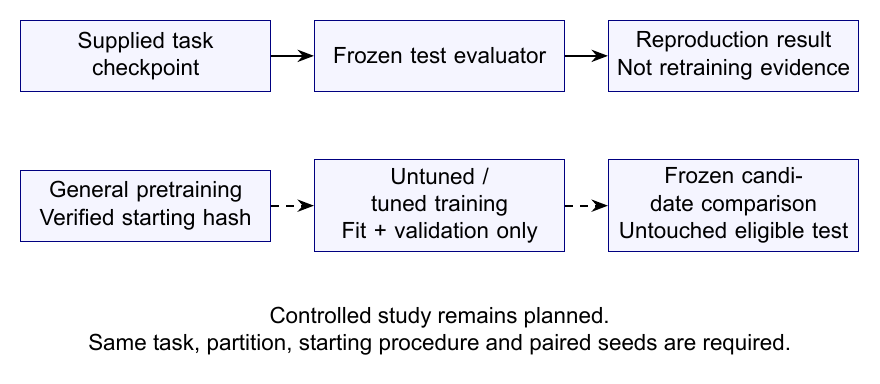
\includegraphics[width=\textwidth]{experiments.png}
\caption{Experiment design.}
\label{fig:experiments}
\floatnote{The upper path reproduces the supplied checkpoint; the lower path is the controlled study, executed in reduced form as shown in Figure~\ref{fig:t41flow}.}
\end{figure}

%-----------------------------------------------------------------------------
\section{Dataset Inspection and Collection}\label{sec:data}

\subsection{IEDXray Audit}
Before any model output was trusted, the supplied IEDXray release was audited.
The audit decoded all 17,360 images and inspected eight annotation files. A
second, read-only preflight of the authorized local copies was run for the T41
study. Table~\ref{tab:audit} summarizes the findings of both. Small numerical
excursions of box coordinates are qualitatively different from semantic label
disagreements and are reported separately. Neither check authorizes a global
label swap or silent clipping of boxes, and the published test data and original
annotations were left unchanged.
\projectrecord{docs/iedxray-audit.md; docs/iedxray-paper-review.md; docs/progress.md}

\begin{table}[htbp]
\centering\tablesetup
\caption{Findings of the IEDXray audit and the T41 preflight.}
\label{tab:audit}
\begin{tabularx}{\textwidth}{@{}YrL{0.36\textwidth}@{}}
\toprule
Finding & Value & Implication\\
\midrule
Images decoded (audit) & 17,360 & Release readable in full\\
Training / test images (preflight) & 12,224 / 5,136 & Matches the published
split\\
Device-label disagreements between exports & 4,955 & Label source must be fixed
per task\\
Distinct boundary findings (audit) & 13 & Reviewed repair needed, no silent
clipping\\
Out-of-image boxes in training exports (preflight) & 5 & Largest overshoot
0.0002745~px\\
Exact-duplicate groups within training & 5 & Keep duplicates in one partition\\
Exact-duplicate groups within test & 112 & Report; test split not altered\\
Exact-byte overlaps between training and test & 4 & Exclude from derived
training data\\
Verified physical-group identifiers & None & Group independence unknown\\
\bottomrule
\end{tabularx}
\end{table}

The preflight findings are bound to the inventory hash
\file{4e5ff81087cc7a7b0bcbbf1abf45806e96ebd7936aca35b583d7f33e471ce9f7}.
They describe the local authorized copies, not an approved partition. The data
owner must confirm the matching inventory on the HPC cluster before derived
training data are created. No repair, partition, training or evaluation was
performed in this step.

\subsection{Collection of Positive X-ray Scans}\label{sec:collection}
The proposal requires a dataset of 500 samples containing positive and negative
scans. The positive scans were collected by the five students in the CVML
laboratory on a dual-energy baggage scanner supplied by Secure Life Group (SLG).
Collection followed the laboratory's multi-bag catalogue, which fixes for every
scan the bag, the threat component and the clutter around it. Each group of the
catalogue occupies four bag slots (A--D), and each slot holds one registered
component from a different family, so that one group distributes a complete set
of IED components over four separate bags (Table~\ref{tab:components}). This
design serves the single-scan task now and the distributed task of SDP~II later.
\projectrecord{docs/meeting_minutes/follow-up-collection-2026-09-28.md}

\begin{table}[htbp]
\centering\tablesetup
\caption{Component families of the collection catalogue.}
\label{tab:components}
\begin{tabularx}{\textwidth}{@{}L{0.24\textwidth}L{0.16\textwidth}Y@{}}
\toprule
Component family & Item codes & Role in an IED\\
\midrule
Explosive simulant & E1--E4 & Main charge\\
Detonator simulant & D1--D3 & Initiator\\
Battery & B1--B3 & Power source\\
Wire & W1--W2 & Electrical connection\\
\bottomrule
\end{tabularx}
\floatnote{All items are labelled laboratory items; explosive and detonator items are simulants.}
\end{table}

Table~\ref{tab:catalogue} summarizes the structure of the catalogue. Every student
was assigned 25 groups (100 bags) over two sessions, so the five students together
cover 125 groups and 500 bag configurations. Each component family appears in
125 configurations, and the catalogue balances five clutter levels and four target
orientations. A structural check of the catalogue confirmed that every group has
four bags with one target from each family.

\begin{table}[htbp]
\centering\tablesetup
\caption{Structure of the Round~1 collection catalogue.}
\label{tab:catalogue}
\begin{tabularx}{\textwidth}{@{}L{0.3\textwidth}Y@{}}
\toprule
Element & Specification\\
\midrule
Configuration group & Four bags (A--D); one explosive simulant, one battery, one
detonator simulant and one wire, each in its own bag with specified clutter\\
Allocation per student & Session~A: 12 groups (48 bags); Session~B: 13 groups (52
bags); 25 groups (100 bags) in total\\
Whole catalogue & 125 groups, 500 bag configurations, 125 per component family\\
Clutter levels & L1--L5, 25 groups (100 bags) each\\
Target orientations & O1--O4, 125 targets each\\
Item variants & All twelve variants of Table~\ref{tab:components}\\
\bottomrule
\end{tabularx}
\end{table}

The collection activity ran from 28~September to 4~November~2026, as reported by the
team. The scan files in the laboratory snapshot are dated 29~September to
9~October~2026. The sessions followed the
schedule agreed with the laboratory (Appendix~\ref{app:management}). The team
completed the 500 catalogue configurations of Round~1. Table~\ref{tab:collection}
gives the snapshot of the laboratory computer taken on 14~November~2026, which
holds 478 distinct image files. The remaining 22 scans are not part of that
snapshot. The snapshot also contains 99 exact copies of existing images in one
storage folder; these are not counted as scans. All 577 files in the snapshot
decoded without error.
\projectrecord{docs/collection-progress-2026-11-14.md}

\begin{table}[htbp]
\centering\tablesetup
\caption{Distinct image files per student.}
\label{tab:collection}
\begin{tabularx}{\textwidth}{@{}L{0.3\textwidth}rY@{}}
\toprule
Student & Distinct files & Scan dates (files)\\
\midrule
Abd Alrahman Ismaik & 142 & 30 Sep (92), 5 Oct (34), 9 Oct (16)\\
Faisal Daoud Alzarooni & 124 & 1 Oct (72), 8 Oct (52)\\
Ahmed Almansoori & 100 & 29 Sep (24), 6 Oct (41), 9 Oct (35)\\
Ali Arif Saeed Alshamsi & 61 & 30 Sep (21), 1 Oct (16), 9 Oct (24)\\
Mohammad Arwani & 51 & 29 Sep (32), 6 Oct (19)\\
\midrule
Total in snapshot & 478 & 29 Sep -- 9 Oct 2026\\
\bottomrule
\end{tabularx}
\floatnote{Laboratory snapshot of 14~November~2026, with the scan dates taken from the file names. The snapshot does not contain all 500 collected scans.}
\end{table}

\subsection{Negative Scans}
Negative (threat-free) scans were collected by the CVML laboratory on the same
SLG-supplied scanner, with assistance from the team. The set contains about
7,000 scans and was shared with the team by the laboratory. The count is
approximate and is reported by the team; the set has not yet been inventoried in
the project repository.

\subsection{Data Handling and Remaining Work}
All scans remain on the laboratory computer. Per-image manifests are kept privately,
and no scan is stored in the public repository. Before the collected data can be
used for training, three steps remain: quality control of each scan, bounding-box
annotation of the targets, and recording of the verified group of each bag so that
related scans stay in the same data split. These steps prepare the data for model
training and for the distributed work of SDP~II.

%-----------------------------------------------------------------------------
\section{Verification Results}\label{sec:verification}

\subsection{Software Checks}
The software is verified at two levels. Automated tests exercise the contracts
and failure handling on synthetic fixtures; they establish software behaviour,
not model accuracy. Table~\ref{tab:checks} lists the checks recorded during
integration on 21~November~2026. The evaluation-enabled run uses the locked root
environment with the evaluator dependencies added:
\begin{center}\small
\texttt{uv run -{}-locked -{}-with-requirements environments/evaluation.in python -m pytest}
\end{center}
Test counts depend on the revision checked and are not a measure of product
quality.

\begin{table}[htbp]
\centering\tablesetup
\caption{Software checks recorded during integration.}
\label{tab:checks}
\begin{tabularx}{\textwidth}{@{}L{0.24\textwidth}L{0.24\textwidth}Y@{}}
\toprule
Checked revision & Result & Scope\\
\midrule
PR~\#18 head \file{6edcd68} & Ruff passed; 273 tests passed & Windows, evaluation
dependencies enabled\\
PR~\#21 head \file{3b5fa3a} & Ruff passed; 286 tests passed & Includes the
integrated evaluator and initialization receipt\\
PR~\#24 merged head \file{87094b1} & Ruff passed; 529 passed, 3 skipped &
Box-repair fixes on top of PR~\#25\\
PR~\#25 head \file{950ea84} & Ruff passed; 525 passed, 3 skipped & Training,
tuning and frozen-test software\\
Required CI & Ubuntu and Windows checks passed & Hosted CPU checks before merge;
no GPU or accuracy evidence\\
\bottomrule
\end{tabularx}
\floatnote{Recorded 21--23~November~2026. All tests use synthetic fixtures.}
\end{table}

\subsection{Diagnostic Inference}
Real inference is a separate level of evidence. The first generic-explosive run
executed the supplied checkpoint on three inspected images on CPU and recorded a
missed modified laptop in the test set; this miss is retained as a known failure.
Later application records describe bounded CPU and CUDA runs for all three
YOLOv10-M tasks. These runs establish that the models execute correctly in the
pipeline; they do not measure benchmark accuracy.

%-----------------------------------------------------------------------------
\section{Evaluation Protocol and Executed Study}\label{sec:protocol}

\subsection{Comparison Modes}
The evaluator supports two comparison modes. A baseline--candidate comparison
measures a tuned model against the supplied checkpoint. A common-parent comparison
measures untuned and tuned models trained from the same starting weights, without
treating one as initialized from the other. A difference between two models is
interpreted as a controlled result only when it is accompanied by training
receipts, paired seeds, the partition identity and comparable training budgets.
The study reported here is a common-parent comparison.

\subsection{Data Policy}
The data policy merged in PR~\#22 and amended in PR~\#25 preserves the published
test split and keeps exact-byte duplicates on the same side of a training-derived
partition. No verified physical groups are available, so that partition is
labelled exploratory and physical independence is not claimed. Five training
boxes that extend less than 0.001~pixels outside their image are clamped in a
derived copy with a change record; the source annotations are never edited, the
published test annotations are never repaired, and larger excursions stay
blocked. The repair accepts only the two published training exports, identified
by their file and content hashes. The shared seed-17 partition contains 9,779
fit images and 2,445 validation images, with every task class on both sides.

\subsection{Executed Study Design}
To fit the report deadline, the owner reduced the original 20-attempt,
three-seed design to the generic-explosive study summarized in
Table~\ref{tab:study} and Figure~\ref{fig:t41flow}. The untuned control used SGD
with an initial learning rate of 0.001, a final learning-rate fraction of 0.01,
weight decay 0.0005 and no mosaic augmentation. The search sampled these four
values; Table~\ref{tab:hyper} compares the control with the selected candidate.
Both 100-epoch confirmations started independently from the same verified
general YOLOv10-M weights, not from a search checkpoint.

\begin{table}[htbp]
\centering\tablesetup
\caption{Design of the executed reduced fine-tuning study (T41).}
\label{tab:study}
\begin{tabularx}{\textwidth}{@{}L{0.26\textwidth}Y@{}}
\toprule
Element & Setting\\
\midrule
Task & Generic explosive detection, one class (category 0)\\
Starting weights & Official general YOLOv10-M (66,924,323 bytes), hash-verified\\
Data & Shared seed-17 partition: 9,779 fit and 2,445 validation images\\
Search & Six attempted configurations of 30 epochs, including the untuned control;
failed attempts count\\
Selection & Validation AP@[.50:.95] after each epoch; test data never used\\
Confirmation & Control and best candidate, 100 epochs each, seed 17\\
Fixed settings & Image size 640, batch 32, FP32, two data-loader workers\\
Hardware & One NVIDIA H100 NVL, four CPUs, 32~GB memory, four-hour job limit\\
Deferred & Specific-explosive task; seeds 29 and 43; full 20-attempt search\\
\bottomrule
\end{tabularx}
\end{table}

\begin{figure}[htbp]\centering
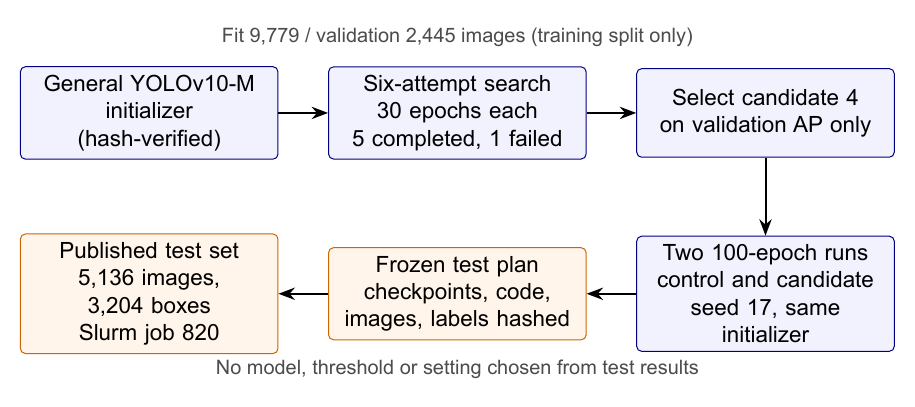
\includegraphics[width=\textwidth]{t41-flow.png}
\caption{Executed T41 study.}
\label{fig:t41flow}
\floatnote{Blue stages use the training split only; orange stages touch the published test set once, after both checkpoints were fixed.}
\end{figure}

\begin{table}[htbp]
\centering\tablesetup
\caption{Hyperparameters of the control and the candidate.}
\label{tab:hyper}
\begin{tabular}{@{}lrr@{}}
\toprule
Hyperparameter & Untuned control & Candidate 4\\
\midrule
Optimizer & SGD & SGD\\
Initial learning rate & 0.001 & 0.000394\\
Final learning-rate fraction & 0.01 & 0.0249\\
Weight decay & 0.0005 & 0.000133\\
Mosaic probability & 0.0 & 0.394\\
\bottomrule
\end{tabular}
\floatnote{Untuned control and selected search candidate. All other settings are identical.}
\end{table}

%-----------------------------------------------------------------------------
\section{Prototype Results: Generic Explosive Detection}\label{sec:results}
This section reports the first measured results of the RayGuard detector. They
come from saved predictions whose metrics a separate process recomputed exactly,
and they are descriptive results for one preselected pair of models trained with
one seed.

\subsection{Search and Confirmation}
Table~\ref{tab:t41jobs} lists every training job. Attempt~0, the untuned
configuration, failed during validation at epoch~6: the pinned detector clipped
predicted boxes lying wholly outside the image to zero area, which the evaluator
rejected. A scoped correction now keeps the original box for such predictions,
and diagnostic and qualification jobs (756 and 757) confirmed that all earlier
predictions and scores were unchanged. The failed attempt still counts against the
budget. The five completed attempts reached validation AP between 86.11\% and
86.99\% after 30 epochs (Figure~\ref{fig:t41search}); attempt~4 was selected.
Successful jobs used 9~h~57~min of GPU time, or 10~h~09~min including the
failure, and every job stayed within its four-hour limit.

\begin{table}[htbp]
\centering\tablesetup
\caption{T41 training jobs.}
\label{tab:t41jobs}
\begin{tabular}{@{}llllr@{}}
\toprule
Stage & Slurm job & Outcome & Elapsed & Val.\ AP\\
\midrule
Search attempt 0 (control) & 755 & Failed at epoch 6 & 0:11:53 & --\\
Search attempt 1 & 758 & 30 epochs & 0:52:41 & 86.81\\
Search attempt 2 & 759 & 30 epochs & 0:52:29 & 86.11\\
Search attempt 3 & 762 & 30 epochs & 0:52:23 & 86.26\\
Search attempt 4 (selected) & 764 & 30 epochs & 0:52:35 & 86.99\\
Search attempt 5 & 767 & 30 epochs & 0:52:34 & 86.18\\
Control confirmation & 770 & 100 epochs; epoch 68 kept & 2:47:35 & 87.71\\
Candidate confirmation & 819 & 100 epochs; epoch 84 kept & 2:46:49 & 87.48\\
\bottomrule
\end{tabular}
\floatnote{Validation AP@[.50:.95] in percent on the training-split validation set.}
\end{table}

\begin{figure}[htbp]\centering
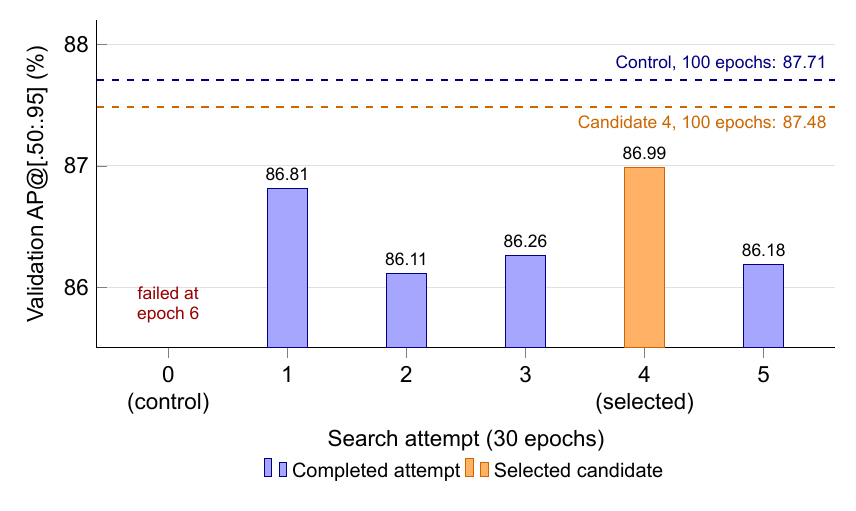
\includegraphics[width=0.9\textwidth]{t41-search.png}
\caption{Validation AP of the search attempts.}
\label{fig:t41search}
\floatnote{Six attempts after 30 epochs and two 100-epoch confirmations (dashed). Attempt 0 failed and has no score.}
\end{figure}

In confirmation, the candidate scored 0.22 percentage points below the control
on validation. The search is too small to show convergence of the Bayesian
sampler: the five sampled attempts all fall within its five random startup
trials. On validation alone,
therefore, tuning showed no benefit.

Figure~\ref{fig:t41curves} shows validation AP after every epoch of the two
confirmation runs. The candidate learned faster during roughly the first 40
epochs, but both runs levelled off at about 87\% after epoch~50 and remained
there; the selected epochs are the maxima of their runs. The plateau indicates
that further epochs alone would not have raised validation AP.

\begin{figure}[htbp]\centering
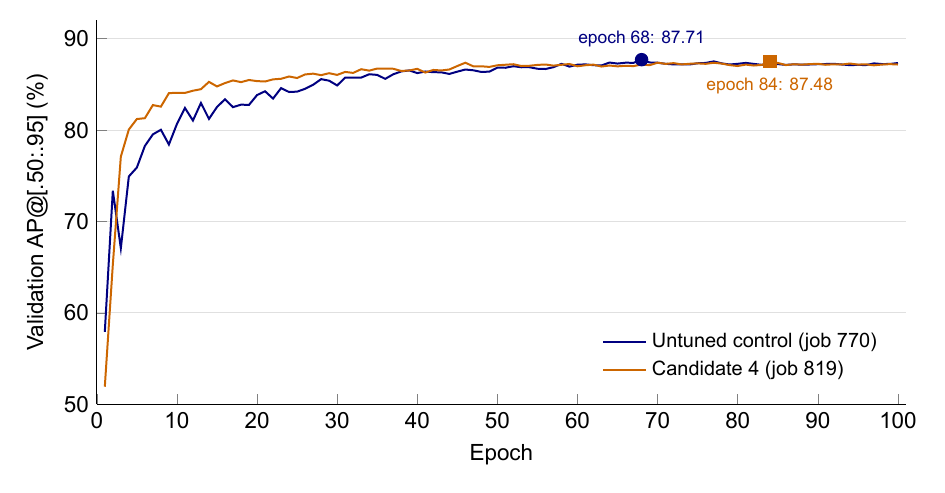
\includegraphics[width=0.95\textwidth]{t41-curves.png}
\caption{Validation AP per epoch of the confirmation runs.}
\label{fig:t41curves}
\floatnote{Two 100-epoch runs; markers show the selected epochs.}
\end{figure}

\subsection{Frozen Test Results}
Before any test image was processed, a test plan fixed the two checkpoints, the
code, the hash of every test image, the original annotations and all settings.
Slurm job~820 then evaluated both models on all 5,136 published test images and
3,204 annotated boxes in 1~min~27~s. Inference used batch size one, FP32, image
size 640, a score floor of 0.001 and at most 300 detections per image; COCO
metrics were computed with pycocotools~2.0.11~\citep{lin2014coco}.
Table~\ref{tab:t41test} gives the results and Figures~\ref{fig:t41test}
and~\ref{fig:t41size} plot them.

\begin{table}[htbp]
\centering\tablesetup
\caption{Frozen test results of the generic detector.}
\label{tab:t41test}
\begin{tabular}{@{}lrrr@{}}
\toprule
Metric & Untuned control & Candidate 4 & Difference\\
\midrule
AP@[.50:.95] & 41.59 & 48.05 & $+6.46$\\
AP@.50 & 63.40 & 66.54 & $+3.14$\\
AP@.75 & 42.29 & 52.35 & $+10.06$\\
AR@1 & 47.33 & 51.91 & $+4.57$\\
AR@100 & 49.26 & 53.27 & $+4.01$\\
\midrule
AP small / medium / large & 33.49 / 35.87 / 47.47 & 27.05 / 43.57 / 53.57 & \\
AR small / medium / large & 50.70 / 46.98 / 51.24 & 37.89 / 51.43 / 56.68 & \\
\midrule
Validation AP@[.50:.95] & 87.71 & 87.48 & $-0.22$\\
\bottomrule
\end{tabular}
\floatnote{Values in percent on the published test set. These are project measurements, not the scores published for IEDXray.}
\end{table}

\begin{figure}[htbp]\centering
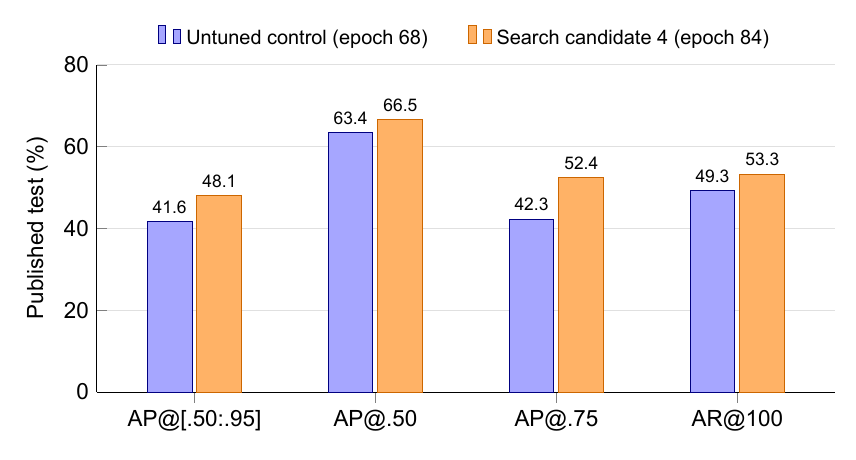
\includegraphics[width=0.9\textwidth]{t41-test.png}
\caption{Test COCO metrics of the control and the candidate.}
\label{fig:t41test}
\floatnote{Published test set; both models were trained for up to 100 epochs from the same starting weights.}
\end{figure}

\begin{figure}[htbp]\centering
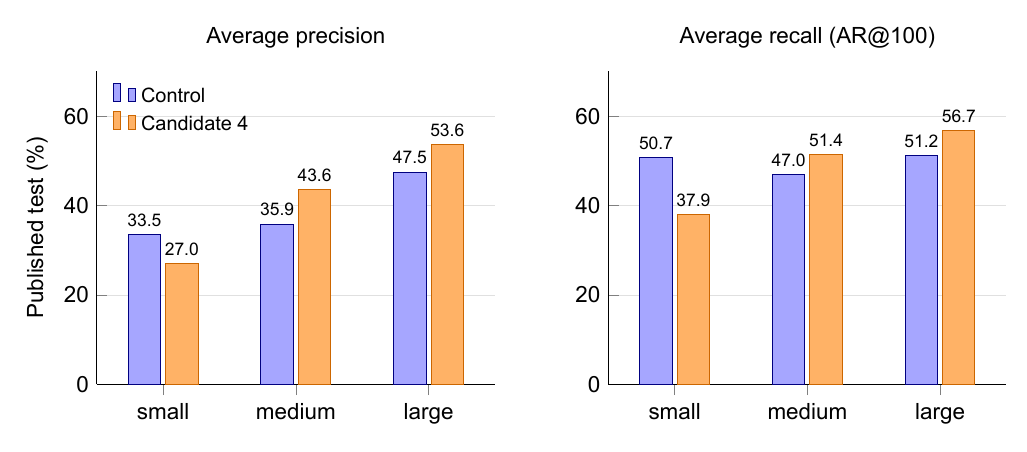
\includegraphics[width=\textwidth]{t41-size.png}
\caption{Test AP and AR by object size.}
\label{fig:t41size}
\floatnote{COCO object sizes on the published test set. The candidate is better on medium and large objects and worse on small ones.}
\end{figure}

The candidate scored 6.46 percentage points higher test AP than the control, with
the largest gain at the stricter IoU of 0.75, which indicates tighter boxes. It
was, however, worse on small objects (AP 27.05\% against 33.49\%, AR 37.89\%
against 50.70\%). Because the candidate was chosen on validation, where it was
slightly worse, the test difference describes this one pair of models; it does
not justify selecting a deployment model after seeing the test scores.

Figure~\ref{fig:t41pr} shows the precision--recall curves behind these AP values,
recomputed from the saved predictions; their averages reproduce AP@.50 and
AP@.75 exactly. At IoU~0.50 the candidate's curve lies above the control's over
almost the whole range, keeping precision above 90\% up to a recall of 0.56
against 0.48 for the control. Both curves end at a recall of 0.70: even at the
lowest score kept (0.001), about 30\% of the annotated threats receive no
matching detection, so lowering the threshold cannot recover them. At the
stricter IoU~0.75 the maximum recall falls to 0.51 and 0.58, which shows that
many detections are found but poorly localized.

\begin{figure}[htbp]\centering
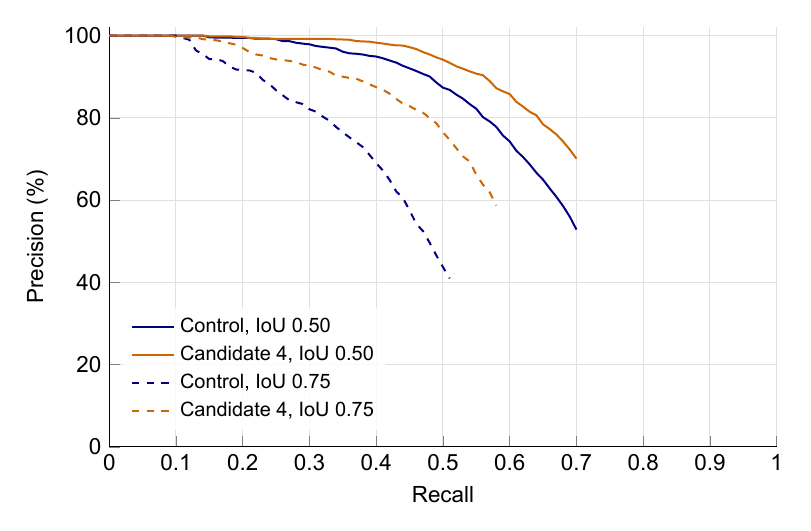
\includegraphics[width=0.85\textwidth]{t41-pr.png}
\caption{Precision--recall curves on the test set.}
\label{fig:t41pr}
\floatnote{IoU 0.50 (solid) and 0.75 (dashed), computed with pycocotools from the saved predictions of job 820. Curves end at the highest recall each model reaches.}
\end{figure}

\subsection{Fixed Operating Point}
An operator sees detections above a confidence threshold, not an AP value. A
threshold of 0.25 with matching at IoU~0.50 was fixed before the test as an
illustrative operating point; it is not optimized or safety-qualified.
Figure~\ref{fig:t41op} and Table~\ref{tab:t41op} show the counts.

\begin{table}[htbp]
\centering\tablesetup
\caption{Detection counts at the fixed operating point.}
\label{tab:t41op}
\begin{tabular}{@{}lrr@{}}
\toprule
Quantity & Untuned control & Candidate 4\\
\midrule
True positives & 1,562 & 1,547\\
False positives & 193 & 80\\
Missed annotated boxes & 1,642 & 1,657\\
False positives on images with no annotation & 55 & 25\\
Precision (\%) & 89.00 & 95.08\\
Recall (\%) & 48.75 & 48.28\\
\bottomrule
\end{tabular}
\floatnote{Confidence 0.25 and IoU 0.50 on the published test set (3,204 annotated boxes).}
\end{table}

\begin{figure}[htbp]\centering
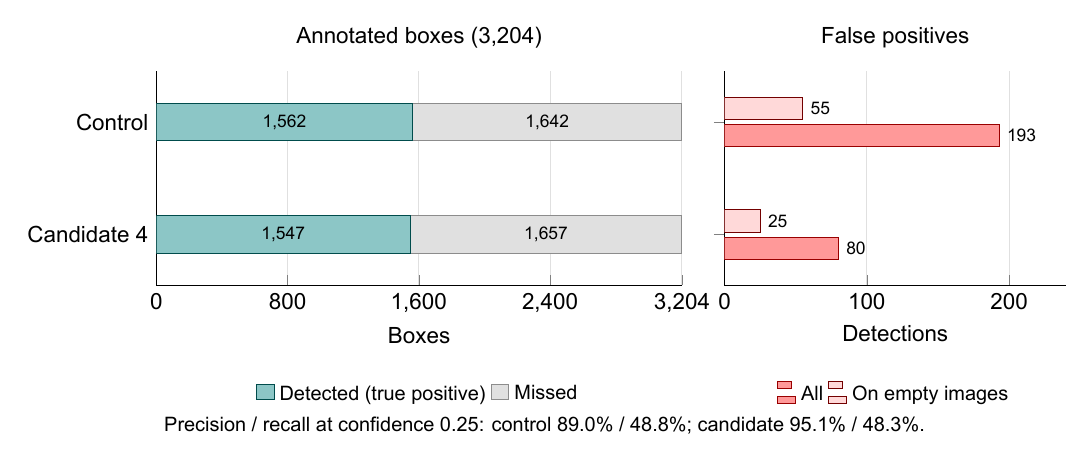
\includegraphics[width=\textwidth]{t41-oppoint.png}
\caption{Detected, missed and false boxes at the operating point.}
\label{fig:t41op}
\floatnote{Left: detected and missed annotated boxes. Right: false positives.}
\end{figure}

At this threshold the candidate produced 59\% fewer false positives, raising
precision from 89.0\% to 95.1\%, but both models detected fewer than half of the
annotated explosives. For a screening aid, a recall below 49\% is the most
important limitation of the prototype: a missed threat is far more costly than a
false alarm that an operator can dismiss. A lower threshold would trade
precision for recall, and choosing it requires a calibration set that is not the
test set.

\subsection{Inspected Examples}
After the evaluation, three test images and their saved predictions were inspected
without changing any model or setting. The selection was descriptive: the first
missed image in order, the candidate's highest-scoring false positive, and an
image already flagged during the audit.
\begin{itemize}
\item \file{Test000001.jpg}: the annotated threat lies over a dense electronic
region. Both models miss it at 0.25; the control's best score is 0.033, and the
candidate produces no detection even at 0.001.
\item \file{Test004918.jpg}: the candidate predicts a region with score 0.945, but
the generic annotation file has no box for this image. It counts as a false
positive against that file; the image is not thereby certified as benign.
\item \file{Test000071.jpg}: the image with the open question over its modified
host label. Both scores are below 0.25 (0.017 and 0.001).
\end{itemize}
Figure~\ref{fig:t41examples} shows the three images with the annotated box and
the models' detections.

\begin{figure}[htbp]\centering
\IfFileExists{figures/private/t41-ex-miss.png}{%
\includegraphics[width=\textwidth]{private/t41-ex-miss.png}\\[2pt]
{\small (a) \file{Test000001.jpg}: missed threat}\\[6pt]
\includegraphics[width=\textwidth]{private/t41-ex-false-positive.png}\\[2pt]
{\small (b) \file{Test004918.jpg}: detection with no annotation}\\[6pt]
\includegraphics[width=\textwidth]{private/t41-ex-label-question.png}\\[2pt]
{\small (c) \file{Test000071.jpg}: open label question}}{%
\fbox{\parbox{0.9\textwidth}{\centering\small The annotated test images are kept
outside the repository. Build them with \file{docs/report/tools/t41_figures.py}
(see \file{docs/report/README.md}).}}}
\caption{Inspected test images.}
\label{fig:t41examples}
\floatnote{Untuned control (left) and candidate~4 (right). Magenta: annotated threat; blue or orange: detection at confidence $\geq 0.25$; grey: the model's highest-scoring detection below 0.25, with its score. Images from the published IEDXray test set~\citep{takele2026iedxray}, reproduced with attribution; overlays added by the team.}
\end{figure}

\subsection{Latency and Resources}
Table~\ref{tab:t41latency} reports inference time on the H100 NVL with batch size
one and FP32, after five warm-up images from the validation set. The predictor
time includes image loading, pre-processing, the model and post-processing; it
excludes input hashing and record writing. At about 7.4~ms per image the
detector is fast enough for interactive use, although the complete operator
workflow, the interface and the scanner hand-off were not timed. The peak GPU
memory allocated by the inference process was 233~MB for the control and
301~MB for the candidate.

\begin{table}[htbp]
\centering\tablesetup
\caption{Inference time per image.}
\label{tab:t41latency}
\begin{tabular}{@{}lrrrr@{}}
\toprule
& \multicolumn{2}{c}{Untuned control} & \multicolumn{2}{c}{Candidate 4}\\
\cmidrule(lr){2-3}\cmidrule(l){4-5}
Timing boundary & Median & p95 & Median & p95\\
\midrule
Predictor call (end to end) & 7.395 & 8.086 & 7.387 & 7.886\\
Model inference only & 5.589 & 5.713 & 5.583 & 5.691\\
\bottomrule
\end{tabular}
\floatnote{Published test set, 5,136 images per model; milliseconds.}
\end{table}

\subsection{Discussion and Limitations}
The prototype detects concealed explosives with moderate accuracy: about half of
the annotated threats are found at the fixed threshold, and the boxes it does
produce are mostly correct. Figure~\ref{fig:t41gap} shows the most important
caveat. Both models scored about 87.5\% AP on the validation set but 41.6\% and
48.1\% on the published test set, a gap of 46.1 and 39.4 percentage points. The validation images come from the same
training split, and without verified physical groups, near-identical scans of the
same bag can appear on both sides of the fit/validation partition, which inflates
validation scores. Four exact-byte overlaps between the published training and
test sets and 112 duplicate pairs inside the test set were deliberately retained
to keep the published split intact. The test score is therefore the more
realistic estimate, but it is not an unseen-case benchmark.

\begin{figure}[htbp]\centering
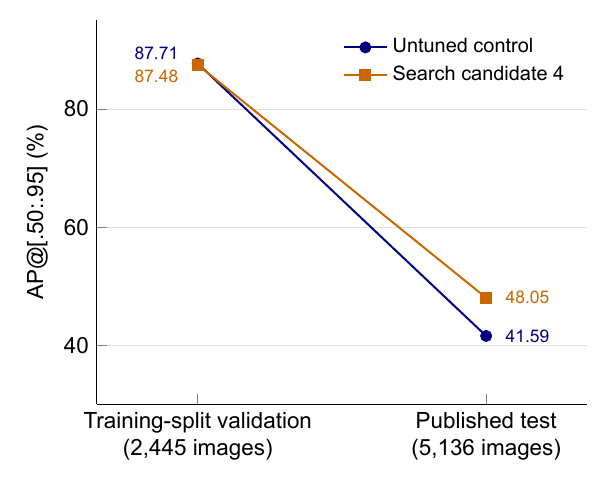
\includegraphics[width=0.62\textwidth]{t41-gap.png}
\caption{Validation and test AP of both models.}
\label{fig:t41gap}
\floatnote{The gaps of 46.1 (untuned) and 39.4 (tuned) percentage points indicate optimistic validation on a split without verified physical groups.}
\end{figure}

The remaining limits follow from the reduced scope. Only one training seed was
used, so no statistical significance or repeatability is claimed. The
specific-explosive task, the full 20-attempt search and the multi-seed study were
deferred. The results concern single-scan generic detection and do not evaluate
host association or threats distributed across several bags. These experiments are
planned for SDP~II (Section~\ref{sec:further}).
\projectrecord{docs/t41-results.md}

%-----------------------------------------------------------------------------
\section{Application Walkthrough}\label{sec:walkthrough}
This section follows one scan through RayGuard-App, from setup to a saved review. The
screenshots were captured on 24~November~2026 from real runs of the application
(application code at revision \file{3488abd}, engine \file{b7ec59e}) on a CPU, at the
fixed threshold of 25\%. Each run took about 12--17~seconds, including the start of the
model process. The scans come from the published IEDXray test
set~\citep{takele2026iedxray}, reproduced with attribution.

\textbf{Model shown.} The screenshots use the YOLOv10-M checkpoints supplied with
IEDXray, not the detector fine-tuned in Section~\ref{sec:results}. The generic
checkpoint has the same architecture, task and output class as the fine-tuned model,
whose weights are not yet integrated in the application. The walkthrough demonstrates
the application and is not evidence of accuracy. The scans were chosen after running
the supplied models on 260 annotated and 60 unannotated test images: two clear
detections, one image without an annotated threat, and the missed threat already shown
in Figure~\ref{fig:t41examples}. None of the four has an exact copy in the training set.

\subsection{Inspecting One Scan}
\begin{enumerate}
\item \textbf{Set up.} The operator chooses an input workflow and a model. The page
shows the model classes, the device and the threshold (Figure~\ref{fig:appsteps}a).
\item \textbf{Load.} A bag scan is uploaded and shown before any detection. Viewing
adjustments change the display only (Figure~\ref{fig:appsteps}b).
\item \textbf{Run.} The operator starts inference explicitly. The scan being processed
is kept apart from the latest completed result (Figure~\ref{fig:appsteps}c).
\item \textbf{Inspect.} The detector marks one region inside the laptop with a score of
91.6\%, linked to its entry in the findings list (Figure~\ref{fig:appresult}).
\item \textbf{Trace.} The provenance tab records the run, threshold, task and checkpoint
hash (Figure~\ref{fig:appsteps}d).
\item \textbf{Review.} The operator adds a note and flags the scan for follow-up. The
application states that a review does not clear or classify the item
(Figure~\ref{fig:appsteps}e).
\item \textbf{Record.} The session page lists every run with its status and review, and
each run can be exported as JSON (Figure~\ref{fig:appsteps}f).
\end{enumerate}

\begin{figure}[htbp]\centering
\IfFileExists{figures/private/app-result.png}{%
\includegraphics[width=\textwidth]{private/app-result.png}}{%
\fbox{\parbox{0.9\textwidth}{\centering\small Screenshots showing dataset scans are kept
outside the repository (see \file{docs/report/README.md}).}}}
\caption{Detection result in RayGuard-App.}
\label{fig:appresult}
\floatnote{IEDXray scan \file{Test001489}~\citep{takele2026iedxray}: one region localized inside the laptop by the supplied generic-explosive checkpoint. The score is not a calibrated probability.}
\end{figure}

\begin{figure}[htbp]\centering
\IfFileExists{figures/private/app-steps.png}{%
\includegraphics[width=\textwidth]{private/app-steps.png}}{%
\fbox{\parbox{0.9\textwidth}{\centering\small Screenshots showing dataset scans are kept
outside the repository (see \file{docs/report/README.md}).}}}
\caption{Walkthrough of one scan.}
\label{fig:appsteps}
\floatnote{(a) Workspace setup, (b) scan loaded, (c) inference running, (d) provenance with checkpoint hash, (e) operator review flagged for follow-up, (f) session records. Supplied generic checkpoint; the navigation sidebar is cropped.}
\end{figure}

\subsection{Comparison with the Reference and Other Tasks}
In dataset replay, the application compares a saved generic result with the published
annotation. Figure~\ref{fig:appcompare} shows two matched threats, an image without an
annotated target and a missed threat. The last two are displayed with the message that an
empty result is not a safety verdict. Table~\ref{tab:appcases} adds the fine-tuned models'
results for the same scans, taken from the saved predictions of job~820 and not produced in
the application. The fine-tuned candidate also finds the laptop threat, but it misses the
walkie-talkie threat that the supplied model finds.

\begin{table}[htbp]
\centering\tablesetup
\caption{Matching scores on the walkthrough scans.}
\label{tab:appcases}
\begin{tabularx}{\textwidth}{@{}L{0.17\textwidth}YL{0.17\textwidth}L{0.15\textwidth}L{0.15\textwidth}@{}}
\toprule
Scan & Content & Supplied model (application) & Control (job 820) & Candidate (job 820)\\
\midrule
\file{Test001489} & Annotated threat in a laptop & 0.916 & 0.968 & 0.954\\
\file{Test002804} & Annotated threat in a walkie-talkie & 0.899 & 0.525 & none (best 0.137)\\
\file{Test003370} & Laptop, no annotated threat & no detection & no detection & no detection\\
\file{Test000001} & Annotated threat over electronics & none & none & none\\
\bottomrule
\end{tabularx}
\floatnote{Highest score at or above 0.25 that matches the annotation with IoU $\geq$ 0.5. Four selected images; not a comparison of model accuracy.}
\end{table}

\begin{figure}[htbp]\centering
\IfFileExists{figures/private/app-compare.png}{%
\includegraphics[width=\textwidth]{private/app-compare.png}}{%
\fbox{\parbox{0.9\textwidth}{\centering\small Screenshots showing dataset scans are kept
outside the repository (see \file{docs/report/README.md}).}}}
\caption{Comparison with the published annotation.}
\label{fig:appcompare}
\floatnote{Annotation in dashed cyan, supplied generic checkpoint in amber: (a) matched threat in a laptop, (b) matched threat in a walkie-talkie, (c) no annotated target and no detection, (d) missed threat.}
\end{figure}

The same scan can be examined with the other supplied tasks
(Figure~\ref{fig:appmodels}). The device model localizes the laptop (91.5\%) and the
specific-explosive model labels the region as a laptop explosive (98.3\%). Both models
passed the application's execution check before use. The application keeps the three
tasks separate and does not combine them into a decision.

\begin{figure}[htbp]\centering
\IfFileExists{figures/private/app-models.png}{%
\includegraphics[width=\textwidth]{private/app-models.png}}{%
\fbox{\parbox{0.9\textwidth}{\centering\small Screenshots showing dataset scans are kept
outside the repository (see \file{docs/report/README.md}).}}}
\caption{One scan with the other supplied checkpoints.}
\label{fig:appmodels}
\floatnote{Scan \file{Test001489}: (a) device detection, (b) specific-explosive detection. Supplied IEDXray checkpoints.}
\end{figure}

\subsection{Interface Evidence from T43}
The interface behaviour around these steps, such as failed runs, filters, unsaved notes
and accessibility, is covered by the eight acceptance tests of RayGuard-App PR~\#1. They
use synthetic images and do not involve a model.

%-----------------------------------------------------------------------------
\section{Application Acceptance}\label{sec:acceptance}
The application is accepted for the demonstration after a dated human rehearsal on
the presentation machine, recording the application and engine revisions. The
rehearsal covers:
\begin{enumerate}
\item a clean start of the application;
\item loading an authorized input image;
\item selecting a model task and obtaining real localizations;
\item reviewing the findings and exporting the record;
\item demonstrating a known miss or error state.
\end{enumerate}
Any pre-recorded fallback must be labelled as recorded. The hand-off of images from
the scanner export and the current application revision also require a dated
acceptance record. No new feature is needed only to generate contribution evidence.

The walkthrough with the fine-tuned checkpoint and a current end-to-end rehearsal remain
open at the date of this report.
